\subsection{Trigonometriske funktioner}
\noindent Vi er nu kommet til at studere trigonometriske funktioner som sinus, cosinus og tangens. For at gøre dette vil vi starte med at betragte vinkler. Man kan måle vinkler i enten radianer eller grader, i dette kursus vil vi oftest benytte radianer, som er et mål for hvor langt man går på enhedscirklen. Vi har følgende sammenhæng mellem grader og radianer
\begin{align*}
2\pi \textup{ rad} = 360 \textup{ grader}
\end{align*}
hvilket medfører at 
\begin{align*}
1 \textup{ rad} = \frac{180}{\pi} \textup{ grader} \qquad \textup{ og } \qquad 1 \textup{ grader} = \frac{\pi}{180} \textup{ rad}.
\end{align*}
\paragraph*{Eksempler:}
\begin{enumerate}
\item Omskriv $2$ radianer til grader:

Vi har 
\begin{align*}
2 \textup{ rad} = 2 \cdot 1 \textup{ rad} = 2 \cdot \frac{180}{\pi} \textup{ grader} = \frac{360}{\pi} \textup{ grader}.
\end{align*}
\item Omskriv $280$ grader til radianer:

Vi har
\begin{align*}
280 \textup{ grader} = 280 \cdot 1 \textup{ grader} = 280 \cdot \frac{\pi}{180} \textup{ rad} = \frac{14\pi}{9} \textup{ rad}.
\end{align*}
\end{enumerate}
For at kunne definere de trigonometriske funktioner vil vi betragte enhedscirklen (se Figur~\ref{fig:funktioner5et}), som er en cirkel med radius $1$ og centrum i origo, som er punktet $(0,0)$.
\begin{figure}
\centering
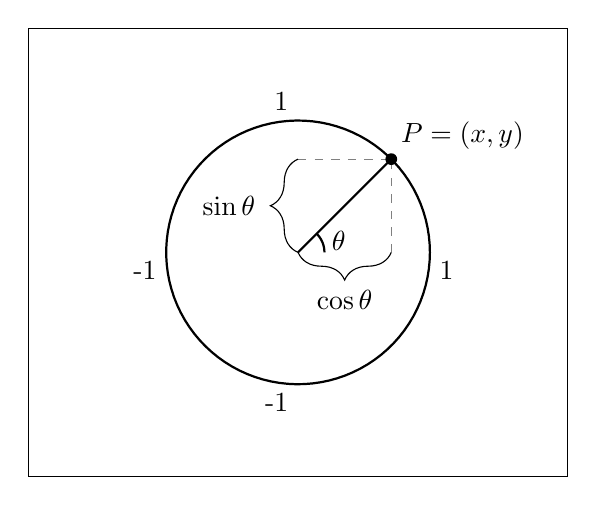
\begin{tikzpicture}
	\begin{axis}[xmin=-1.7,xmax=1.7,ymin=-1.7,ymax=1.7,ticks=none,axis equal]
	\addplot[domain=0:2*pi,thick, samples=100] ({cos(deg(x))},							{sin(deg(x))});
	\addplot[domain=0:sqrt(2)/2,thick] {1*x};
	\addplot[domain=0:pi/4,thick,samples=200] ({0.2*cos(deg(x))},						{0.2*sin(deg(x))})node[right,pos=0.6] {$\theta$};
	\node[above left] at (axis cs:0,1) {1};
	\node[below right] at (axis cs:1,0) {1};
	\node[below left] at (axis cs:0,-1) {-1};
	\node[below left] at (axis cs:-1,0) {-1};
	\draw[gray,dashed] (axis cs:{sqrt(2)/2},0) -- (axis cs:{sqrt(2)/2},{sqrt(2)/2});
	\draw[gray,dashed] (axis cs:0,{sqrt(2)/2}) -- (axis cs:{sqrt(2)/2},{sqrt(2)/2});
\draw [decorate,decoration={brace,amplitude=10pt}]
(axis cs:{sqrt(2)/2},0) -- (axis cs:0,0)node [below=10pt,midway] {$\cos\theta$};
\draw [decorate,decoration={brace,amplitude=10pt}]
(axis cs:0,0) -- (axis cs:0,{sqrt(2)/2})node [left=12pt,midway] {$\sin\theta$};
\node[fill,circle,inner sep=1.5pt] at (axis cs:{sqrt(2)/2},{sqrt(2)/2}){};
\node[above right] at (axis cs:{sqrt(2)/2},{sqrt(2)/2}){$P=(x,y)$};

\end{axis}
\end{tikzpicture}
\caption{Sinus og cosinus i enhedscirklen.}
\label{fig:funktioner5et}
\end{figure}
Hvis vi starter i punktet $(1,0)$ på enhedscirklen og bevæger os med en vinkel $\theta$ mod uret (se Figur~\ref{fig:funktioner5et}) så når vi til et punkt på enhedscirklen som vi kalder $P$. Hvis $P$ har koordinaterne $(x,y)$ så definerer vi $\cos\theta=x$ og $\sin\theta=y$. Hvis vi går imod urets retning i enhedscirklen, vil vi kalde det for den positive omløbsretning og hvis vi går i urets retning, vil vi kalde det for den negative omløbsretning.

Bemærk, at enhedscirklen er $2\pi$-periodisk. Det betyder, at hvis vi går en vinkel på $\theta$ mod uret og får et punkt $P$, så vil vi få det samme punkt hvis vi går vinklen $\theta+2\pi$, da der er $2\pi$ rundt om hele enhedscirklen. Det medfører også at sinus og cosinus er $2\pi$-periodiske funktioner, hvilket betyder at
\begin{align*}
\sin\theta = \sin(\theta + 2\pi k) \qquad \textup{ og } \qquad \cos\theta = \cos(\theta + 2\pi k),
\end{align*}
hvor $k$ er et heltal.

Hvis vi betragter Figur~\ref{fig:funktioner5to} ser vi, at hvis vi spejler et punkt $(x,y)$, på enhedscirklen, omkring $x$-aksen får vi punktet $(x,-y)$ på enhedscirklen. Da det at spejle et punkt omkring $x$-aksen er det samme som at gå vinklen i den negative omløbsretning, får vi at 
\begin{align*}
\sin(-\theta) = -\sin\theta \qquad \textup{ og } \qquad \cos(-\theta)=\cos\theta.
\end{align*}
På tilsvarende vis ser vi, at hvis vi spejler punktet $(x,y)$ i $y$-aksen får vi punktet $(-x,y)$. Da det at spejle i $y$-aksen, er det samme som at gå vinklen $\pi - \theta$ i positiv omløbsretning får vi, at
\begin{align*}
\sin(\pi - \theta)=\sin\theta \qquad \textup{ og } \qquad \cos(\pi - \theta) = - \cos\theta.
\end{align*} 
Vi definerer nu tangens ud fra sinus og cosinus, ved
\begin{align*}
\tan\theta=\frac{\sin\theta}{\cos\theta},
\end{align*}
når $\theta \neq \frac{\pi}{2} + \pi k$, hvor $k$ er et heltal. Tangens kan også bestemmes ud fra enhedscirklen (se Figur~\ref{fig:funktioner5tre}). Vi tegner en tangentlinje der skærer cirklen i punktet $(1,0)$. Hvis vi går en vinkel $\theta$ i enhedscirklen og så forlænger linjen indtil den skærer vores tangent, så er $\tan\theta$ præcis $y$-koordinaten i skæringspunktet. 
\begin{figure}[!htbp]
\begin{minipage}{0.49\textwidth}
\centering
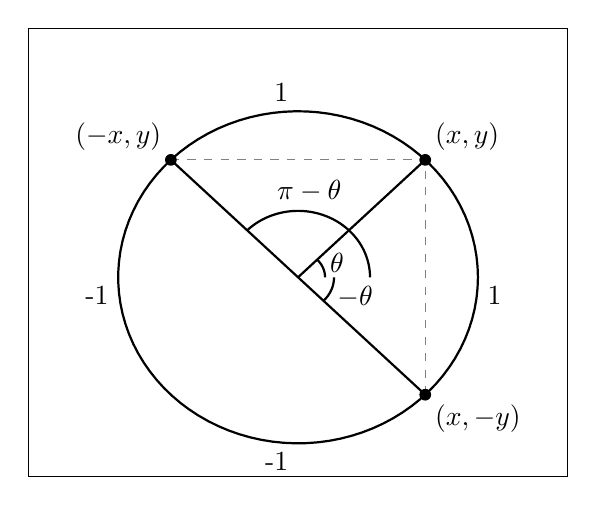
\begin{tikzpicture}
	\begin{axis}[xmin=-1.5,xmax=1.5,ymin=-1.2,ymax=1.5,ticks=none]
	\addplot[domain=0:2*pi,thick, samples=100] ({cos(deg(x))},							{sin(deg(x))});
	\addplot[domain=0:sqrt(2)/2,thick] {1*x};
	\addplot[domain=-sqrt(2)/2:sqrt(2)/2,thick] {-1*x};
	\addplot[domain=0:pi/4,thick,samples=200] ({0.15*cos(deg(x))},						{0.15*sin(deg(x))})node[right,pos=0.8] {$\theta$};
	\addplot[domain=0:-pi/4,thick,samples=200] ({0.2*cos(deg(x))},						{0.2*sin(deg(x))})node[right,pos=0.8] {$-\theta$};
	\addplot[domain=0:3*pi/4,thick,samples=200] ({0.4*cos(deg(x))},						{0.4*sin(deg(x))})node[above,pos=0.6] {$\pi-\theta$};
	\node[above left] at (axis cs:0,1) {1};
	\node[below right] at (axis cs:1,0) {1};
	\node[below left] at (axis cs:0,-1) {-1};
	\node[below left] at (axis cs:-1,0) {-1};
	\draw[gray,dashed] (axis cs:{sqrt(2)/2},{-sqrt(2)/2}) -- (axis cs:{sqrt(2)/2},{sqrt(2)/2});
	\draw[gray,dashed] (axis cs:{-sqrt(2)/2},{sqrt(2)/2}) -- (axis cs:{sqrt(2)/2},{sqrt(2)/2});
%\draw [decorate,decoration={brace,amplitude=10pt}]
%(axis cs:{sqrt(2)/2},0) -- (axis cs:0,0)node [below=10pt,midway] {$\mathrm  {cos}(\theta)$};
%\draw [decorate,decoration={brace,amplitude=10pt}]
%(axis cs:0,0) -- (axis cs:0,{sqrt(2)/2})node [left=12pt,midway] {$\mathrm  {sin}(\theta)$};
\node[fill,circle,inner sep=1.5pt] at (axis cs:{sqrt(2)/2},{sqrt(2)/2}){};
\node[above right] at (axis cs:{sqrt(2)/2},{sqrt(2)/2}){$(x,y)$};
\node[fill,circle,inner sep=1.5pt] at (axis cs:{sqrt(2)/2},{-sqrt(2)/2}){};
\node[below right] at (axis cs:{sqrt(2)/2},{-sqrt(2)/2}){$(x,-y)$};
\node[fill,circle,inner sep=1.5pt] at (axis cs:{-sqrt(2)/2},{sqrt(2)/2}){};
\node[above left] at (axis cs:{-sqrt(2)/2},{sqrt(2)/2}){$(-x,y)$};
\end{axis}
\end{tikzpicture}
\caption{Symmetrien i enhedscirklen.}
\label{fig:funktioner5to}
\end{minipage}
\begin{minipage}{0.49\textwidth}
 \centering
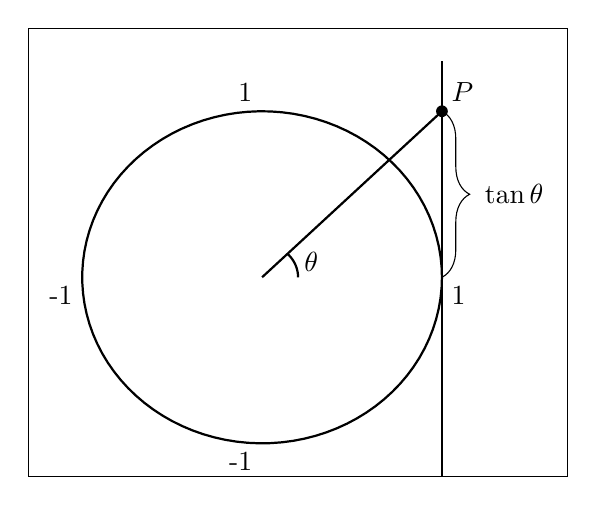
\begin{tikzpicture}
	\begin{axis}[xmin=-1.3,xmax=1.7,ymin=-1.2,ymax=1.5,ticks=none]
	\addplot[domain=0:2*pi,thick, samples=100] ({cos(deg(x))},							{sin(deg(x))});
	\addplot[domain=0:1,thick] {1*x};
	\addplot[domain=0:pi/4,thick,samples=200] ({0.2*cos(deg(x))},						{0.2*sin(deg(x))})node[right,pos=0.6] {$\theta$};
	\node[above left] at (axis cs:0,1) {1};
	\node[below right] at (axis cs:1,0) {1};
	\node[below left] at (axis cs:0,-1) {-1};
	\node[below left] at (axis cs:-1,0) {-1};
\draw[thick] (axis cs:1,-1.3) -- (axis cs:1,1.3);
\draw [decorate,decoration={brace,amplitude=10pt}]
(axis cs:1,1) -- (axis cs:1,0)node [right=12pt,midway] {$\tan\theta$};
\node[fill,circle,inner sep=1.5pt] at (axis cs:1,1){};
\node[above right] at (axis cs:1,1){$P$};
\end{axis}
\end{tikzpicture}
\caption{Tangens i enhedscirklen.}
\label{fig:funktioner5tre}
\end{minipage}
\end{figure}
\paragraph*{Trigonometriske identiter}
Vi opsummere her en liste over de trigonometriske identiteter vi har vist plus nogle flere som vil være brugbare i opgaveregningen:
\begin{enumerate}
\item $\cos(\theta + 2\pi k) = \cos(\theta)$, når $k$ er et heltal.
\item $\sin(\theta + 2\pi k) = \sin(\theta)$, når $k$ er et heltal.
\item $\sin(-\theta)=-\sin(\theta)$.
\item $\cos(-\theta)=\cos(\theta)$.
\item $\sin(\pi \pm \theta)=\mp \sin(\theta)$.
\item $\cos(\pi \pm \theta)=-\cos(\theta)$.
\item $\tan(\pi \pm \theta)=\pm \tan(\theta)$.
\item $\cos^2(\theta) + \sin^2(\theta)=1$ (Idiotformlen).
\item $\sin(\theta \pm \phi) = \sin(\theta)\cos(\phi)\pm\cos(\theta)\sin(\phi)$ (Additionsformlen for sinus).
\item $\cos(\theta \pm \phi) = \cos(\theta)\cos(\phi)\mp\sin(\theta)\sin(\phi)$ (Additionsformlen for cosinus).
\item $\cos(2\theta)=\cos^2(\theta)-\sin^2(\theta) = 2\cos^2(\theta)-1 = 1-2\sin^2(\theta)$.
\item $\sin(2\theta)=2\sin(\theta)\cos(\theta)$.
\end{enumerate}
Derudover giver vi en liste over værdierne for nogle udvalgte vinkler. Vi betragter her kun vinkler i første kvadrant, da vi kan finde værdier for de andre kvadranter ved at benytte de ovenstående formler.

\begin{table}[h!]
\centering
\begin{tabular}{l !{\qquad} {c}!{\qquad} {c}!{\qquad} r}
$\theta$           & $\sin \theta$ & $\cos \theta$ & $\tan \theta$  \\
\toprule
$0$				 & $0$ 				    & $1$  				   & $0$					\\ \midrule
$\displaystyle \frac{\pi}{6}$  & $\displaystyle\frac{1}{2}$        & $\displaystyle\frac{\sqrt{3}}{2}$ & $\displaystyle \frac{\sqrt{3}}{3}$   \\ \midrule
$\displaystyle\frac{\pi}{4}$  & $\displaystyle\frac{\sqrt{2}}{2}$	& $\displaystyle\frac{\sqrt{2}}{2}$ &	$1$					\\ \midrule
$\displaystyle\frac{\pi}{3}$  & $\displaystyle\frac{\sqrt{3}}{2}$ & $\displaystyle\frac{1}{2}$		   & $\sqrt{3}$				\\ \midrule
$\displaystyle\frac{\pi}{2}$  & $1$ 			        & $0$				   &   \\
\bottomrule  
\end{tabular}
\caption{Værdier for udvalgte vinkler}\label{tab:funktioner5et}
\end{table}

\paragraph*{Eksempler:}
\begin{enumerate}
\item Beregn værdien $\cos(\frac{3\pi}{2})$:

Ved at bruge den trigonometriske identitet nummer $6.$ får vi at
\begin{align*}
\cos\Big( \frac{3\pi}{2}\Big) = \cos\Big(\pi + \frac{\pi}{2}\Big) = -\cos\Big(\frac{\pi}{2} \Big)=-0=0.
\end{align*}
\item Beregn $\sin(9\pi)$:

Ved at bruge den trigonometriske identitet nummer $2.$ får vi at
\begin{align*}
\sin(9\pi)=\sin(\pi + 8\pi)= \sin(\pi + 2 \cdot 4 \cdot \pi) = \sin(\pi) = 0.
\end{align*}
\item Vis at den trigonometriske identitet nummer $5$. gælder for plus, ved at bruge additionsformlen for sinus:

Vi sætter $\phi=\pi$ i additionsformlen for sinus og får
\begin{align*}
\sin(\theta+\pi) = \sin(\theta)\cos(\pi)+\cos(\theta)\sin(\pi).
\end{align*}
Vi ser i enhedscirklen at~\ref{tab:funktioner5et} at $\cos(\pi)=-1$ og $\sin(\pi)=0$. Indsætter vi det i den ovenstående ligning får vi at
\begin{align*}
\sin(\theta+\pi) = \sin\theta\cdot (-1)+\cos\theta\cdot 0 =-\sin\theta.
\end{align*}
\end{enumerate}